\chapter{Metodologia}
\label{chap:metodologia}
\thispagestyle{empty}

É apresentado neste capitulo o desenvolvimento realizado neste projeto, os problemas encontrados e as soluções propostas.
Na primeira e segunda seção tem-se a definição do modelo matemático do veiculo protótipo DT1 e da pista. A terceira seção traz a formulação proposta para o problema de controle ótimo que encontrar
a estrategia de pista ótima. Por fim, na ultima seção é apresentado os passos realizados no desenvolvimento do código que soluciona o OPC proposto. 

\section{Modelo do veiculo DT1} 

O modelo da dinâmica do veiculo protótipo DT1 foi definido com base na revisão bibliográfica apresentada na Seção \ref{sec:modelo}. 
Para isto as seguintes simplificações e considerações foram feita:

\begin{itemize}
    \item \textbf{Dinâmica lateral:} não foi levando em conta a dinâmica lateral do veiculo considerando que ele se move apenas em linha reta; 
    \item \textbf{Vento:} a velocidade do vento foi desconsiderada na Equação (\ref{eq:Fa});
    \item \textbf{Pneus:} a variação do coeficiente de rolamento em funça da temperatura, da pressão e a velocidade não foi considerada na Equação (\ref{eq:Fr});
    \item \textbf{Rolamentos:} o atrito viscos dos rolamentos foi considerado nulo;
    \item \textbf{Perdas elétricas:} a bateria e o conversor eletrônico de potencia foram tratados como componentes ideias não modificações na dinâmica das grandezas elétricas;
    \item \textbf{Indutância do motor:} como o dinâmica da velocidade é pelo menos dez vez mais lenta que a dinâmica da corrente elétrica, a contribuição do do indutor foi removida da Equação (\ref{eq:propulsao_1}).  
\end{itemize}

A partir das Equações (\ref{eq:SomaForcas}) à (\ref{eq:Fr}) e (\ref{eq:propulsao}) e destas simplificações e considerações foi definido a 
seguinte equação para descrever o comportamento do veiculo

\begin{subequations}
	\label{eq:modelo_1}
    \begin{align}
        (m_v + m_p + N_r \cdot \frac{J_r}{r_r^2}  + \frac{J_m}{r_m^2}) \dot v = F_t - (F_a + F_g + F_r) \enspace,\\   
        F_{t} =  \frac{K_t \cdot i_a \cdot \eta}{r_m} \enspace,\\
		R_{a} \cdot i_{a} = u - \frac{K_{v} \cdot v}{r_m} \enspace, \\
        F_{a} = \frac{\rho \cdot a_f \cdot c_d \cdot v^2}{2} \enspace,\\
        F_{g} = (m_v + m_p) \cdot g \cdot \sin(\theta(x)) \enspace,\\
        F_{r}  = c_{r} \cdot (m_v + m_p) \cdot g \cdot \cos(\theta(x)) \enspace,
	\end{align}
\end{subequations}

em que as variáveis são $\dot v$ a aceleração 
do carro em [$m/s^2$], $v$ a velocidade do carro em [$m/s^2$], $x$ a distancia percorrida pelo carro na pista em [$m$], 
$u$ a tensão aplicada no motor em [$V$], $r_m$ o raio do cilindro de transmissão no eixo do motor elétrico em [$m$] e $\theta$ é a inclinação da pista em [$rad$] 
e as constantes estão apresentadas na Tabela \ref{tab:constantes}. Não foi realizado ensaio para determinar ou verificar essas constantes e este modelo
pois o projeto foi realizado, em sua maior parte, durante o Ensino Remoto Emergêncial de 2020. As constantes foram definidas através da bibliografia apresentada
e por dados fornecidos pela equipe Milhagem UFMG. 

% em que as variáveis são $u$ a tensão aplicada no motor em [$V$], 
% $r_m$ o raio do cilindro de transmissão no eixo do motor em [$m$], 
% $\theta$ é a inclinação da pista em [$rad$], $\dot v$, $v$ e $x$ são respectivamente a aceleração em [$m/s^2$], a velocidade em [$m/s$] e posição [$m$] do carro
% e as constantes estão apresentadas na Tabela \ref{tab:constantes}. Não foi realizado ensaio para determinar ou verificar essas constantes ou este modelo
% pois o projeto foi realizado, em sua maior parte, durante o Ensino Remoto Emergêncial. As constantes foram definidas através da bibliografia apresentada
% e por dados fornecidos pela equipe Milhagem UFMG. 

\begin{table}[H]
	\centering
	\caption{Constantes utilizadas no modelo do veiculo}
	\rowcolors{1}{}{lightgray}
	\begin{tabular}{llll}
		\toprule
		\textbf{Constante} & \textbf{Simbolo} & \textbf{Unidade} & \textbf{Valor}\\
		\hline
		Massa veiculo                       & $m_v$  & [$kg$]              & 36      \\
        Massa do piloto                     & $m_p$  & [$kg$]              & 50      \\
        Resistência de armadura             & $R_a$  & [$\Omega$]        & 0,07    \\  
        Const. de tensão induzida           & $K_v$  & [$V/(rad/s)$]       & 0,119   \\
        Quantidade de rodas                 & $N_r$  & [ ]                & 3       \\
        Momento de inercia da roda          & $J_r$  & [$kg.m^2$]        & 0,015   \\
        Momento de inercia do motor         & $J_m$  & [$kg.m^2$]        & $0,0625 \times 10^{-3}$\\
        Raio da roda                        & $r_r$  & [$m$]               & 0,254   \\
        Const. de torque                    & $K_t$  & [$Nm/A$]            & 0,119   \\
        Eficiencia da roda de atrito        & $\eta$ & [ ]                & 0,95    \\
        Densidade do ar                     & $\rho$ & [$kg/m^3$]        & 1,22    \\
        Areá fronta do veiculo              & $a_f$  & [$m^2$]           & 0,26    \\
        Coef. de arrasto aerodinamico       & $c_d$  & [ ]                & 0,164   \\
        Aceleração da gravidade             & $g$    & [$m/s^2$]         & 9,81    \\
        Coef. de resistência ao rolamento   & $c_r$  & [ ]                & 0,0024  \\
		\bottomrule
	\end{tabular}
	\caption*{\footnotesize Fonte: Elaborada pelo autor.}
	\label{tab:constantes}
\end{table}


\section{Modelo da pista}

Para obter os dados de altitude da pista da Shell Eco-marathon Americas de 2019 no Kartódromo de Sonoma foi feito uma requisição a equipe
equipe \textit{Duke Electric Vehicles} da \textit{Duke University} que disponibilizou os dados coletados e tratos por ela. A Figura apresentada \ref{fig:altitude_pista} 
o perfil de altitude da pista com estes dados.

\begin{figure}[h]
    \centering
    \caption{Perfil de altitude da pista da Shell Eco-marathon Americas de 2019}
    % This file was created by matlab2tikz.
%
%The latest updates can be retrieved from
%  http://www.mathworks.com/matlabcentral/fileexchange/22022-matlab2tikz-matlab2tikz
%where you can also make suggestions and rate matlab2tikz.
%
\definecolor{mycolor1}{rgb}{0.00000,0.44700,0.74100}%
%
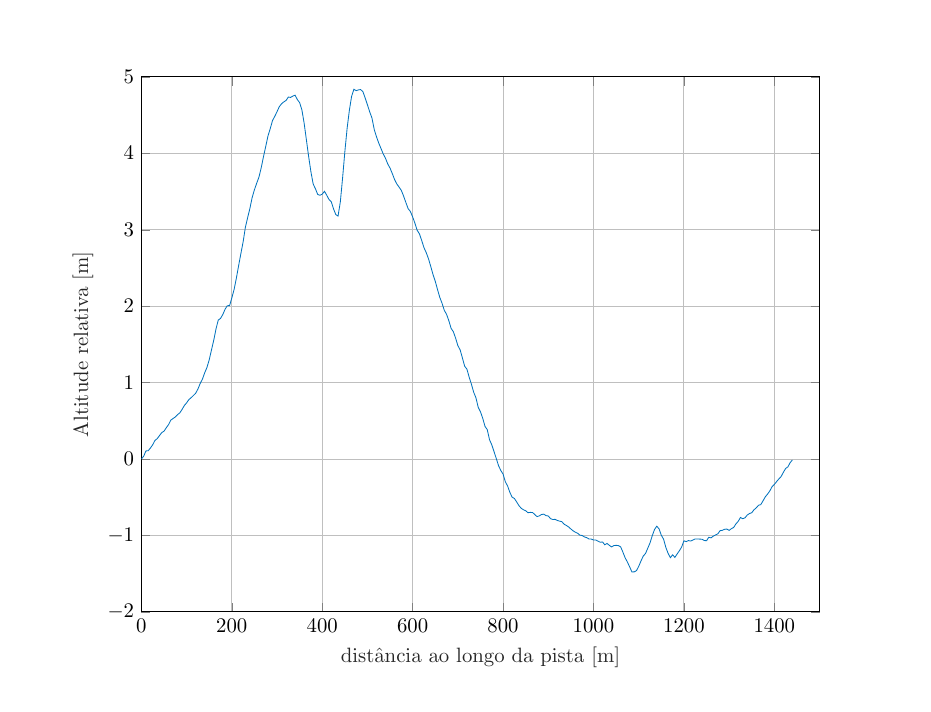
\begin{tikzpicture}[scale=0.75]

\begin{axis}[%
width=4.521in,
height=3.566in,
at={(0.758in,0.481in)},
scale only axis,
xmin=0,
xmax=1500,
xlabel style={font=\color{white!15!black}},
xlabel={distância  ao longo da pista [m]},
ymin=-2,
ymax=5,
ylabel style={font=\color{white!15!black}},
ylabel={Altitude relativa [m]},
axis background/.style={fill=white},
xmajorgrids,
ymajorgrids,
/pgf/number format/.cd,
        use comma,
        1000 sep={}
]
\addplot [color=mycolor1, forget plot]
  table[row sep=crcr]{%
0	0\\
5.12221633837888	0.0357379396676334\\
10.0516199164945	0.104972074967328\\
15.1016863618342	0.107722115067246\\
20.0557383939357	0.143408459194609\\
25.0180390039261	0.185390922437452\\
30.0994558692112	0.242808963848907\\
35.0194754612144	0.265343842059095\\
40.1032362448675	0.306213896817238\\
45.0302720648865	0.34432100835364\\
50.0199618336967	0.363243823798147\\
55.0601872298759	0.408402295729659\\
60.081861665023	0.448736973032622\\
65.0034315382065	0.507448710411661\\
70.0133461222134	0.528655675550714\\
75.0427696663329	0.548738481850909\\
80.0289031360195	0.580077859552539\\
85.0540374361473	0.603092814287619\\
90.0039519341915	0.647564873838286\\
95.0344626775333	0.699131894236861\\
100.08412719663	0.734374644606736\\
105.087949763056	0.776654148548195\\
110.029320108579	0.801470868883285\\
115.109002769075	0.830801204323592\\
120.047990525275	0.859470217807589\\
125.077509699709	0.91471428857013\\
130.043700015891	0.986995023844734\\
135.057777483852	1.04455129324355\\
140.023845274091	1.12650442548788\\
145.067814961286	1.1975924169145\\
150.071951699855	1.29765754647297\\
155.067333935021	1.42611842181642\\
160.046476069651	1.55343586345637\\
165.024396395583	1.70034960164136\\
170.059139443888	1.81757768174917\\
175.033685409674	1.83842327477578\\
180.100556336227	1.88992242741691\\
185.093553265802	1.95895970651273\\
190.075606815513	2.00573333352113\\
195.072302587681	2.00650260273968\\
200.084744663884	2.1076074957122\\
205.046000450717	2.21707009877046\\
210.03864921318	2.36430784814989\\
215.098558493801	2.52909944692323\\
220.067805214036	2.68727014749316\\
225.104324773213	2.84193460225021\\
230.05185929419	3.03165841315539\\
235.077383866855	3.15829537724148\\
240.017508877014	3.27837165636326\\
245.005808937912	3.42016227481439\\
250.015268947595	3.52188807387367\\
255.050892541585	3.60834889388607\\
260.0063277381	3.68748899725192\\
265.001156445286	3.80818363772489\\
270.070454536791	3.95485125560833\\
275.015227568311	4.08844028589769\\
280.07919560007	4.22764024171798\\
285.072102690404	4.32337923819937\\
290.088508702335	4.42913326069625\\
295.020995241378	4.48294754669859\\
300.057050371967	4.54487313347786\\
305.071971070169	4.60995547396562\\
310.067857483967	4.6480347286057\\
315.047026372111	4.67283089060249\\
320.011218889021	4.6916842630321\\
325.045486563677	4.73623001881343\\
330.005090294992	4.73121711204915\\
335.084013035874	4.74915299856471\\
340.005128438622	4.76033344145669\\
345.046186095374	4.70260303614258\\
350.059781945331	4.66277010581372\\
355.037249011958	4.56879524739148\\
360.088602713913	4.39077246022415\\
365.046961987169	4.17467114933649\\
370.01071293774	3.95628631039429\\
375.04960497426	3.75611837613893\\
380.013235457204	3.5983623827951\\
385.010028062919	3.53529426275642\\
390.024258467701	3.46152316489486\\
395.073752715841	3.4504967877954\\
400.100767589134	3.4657282840199\\
405.044216785212	3.50316296864385\\
410.046252351497	3.45107272053722\\
415.003397910249	3.39522146375892\\
420.068346926989	3.36561232213679\\
425.00814024125	3.27320493082273\\
430.018228184296	3.19784489867244\\
435.033185395297	3.17867482035181\\
440.062335167934	3.36366439572127\\
445.067880453611	3.67678539727011\\
450.112944370747	4.02373555328033\\
455.11403031075	4.32732894090232\\
460.031288489432	4.56208775403152\\
465.01377484305	4.74555059404158\\
470.094421755121	4.83813648123462\\
475.007478345653	4.81994370474145\\
480.093488339411	4.8294559666483\\
485.000116654387	4.8345701495991\\
490.093619430145	4.80574940639705\\
495.087218007541	4.72226349670508\\
500.086065915516	4.63320429294828\\
505.104190099561	4.54126835063877\\
510.019711436402	4.46206553739806\\
515.048889261962	4.31136925109454\\
520.050480466514	4.21620789363706\\
525.012290421834	4.13402072221267\\
530.040185205617	4.06237307599751\\
535.013378599529	3.99088064611747\\
540.003754990435	3.93460579828708\\
545.081387320683	3.85947030304406\\
550.11616167678	3.80514844662332\\
555.10335455619	3.7335202568295\\
560.090760735292	3.65628812843982\\
565.018483478686	3.59900863087375\\
570.063865000408	3.55724806163802\\
575.087323611412	3.51314509373265\\
580.07577584618	3.43907631088358\\
585.003009891568	3.35668016868912\\
590.013775544679	3.27571958492176\\
595.053529786038	3.23793714976627\\
600.023704620358	3.16736800714642\\
605.081284173436	3.08484077108421\\
610.024102859829	2.99222287368472\\
615.003442302492	2.94648330432707\\
620.019195038574	2.85930067853677\\
625.106885313401	2.76507427978904\\
630.079658274351	2.69969907593198\\
635.079625831954	2.61986156018748\\
640.018038586473	2.52039761917368\\
645.040866697825	2.41451099895905\\
650.067821212943	2.32463779545542\\
655.003093402256	2.21811729440853\\
660.057310505983	2.11457052992626\\
665.023052254712	2.03802093262931\\
670.058568408263	1.94486754473429\\
675.053678819237	1.89254797025235\\
680.089975845145	1.80918873004759\\
685.080739434188	1.70896309716183\\
690.039547759312	1.66520815629269\\
695.04128133922	1.58163176026549\\
700.01571840371	1.48361138379975\\
705.100318245575	1.42705947673011\\
710.019961384519	1.32367399862178\\
715.004297485676	1.21468583866631\\
720.109323670961	1.17472385243005\\
725.084032125554	1.06928976180669\\
730.023660108317	0.97829622998816\\
735.020965856036	0.873257703766727\\
740.005772883376	0.800793016734662\\
745.055880794773	0.675465616374825\\
750.08620183061	0.616332205593579\\
755.063882098672	0.531733627663317\\
760.079998487305	0.425911531812245\\
765.00088746981	0.384668536036159\\
770.100450999183	0.250972178052027\\
775.036344554228	0.185002672519197\\
780.100972351368	0.0944669917970231\\
785.110777356283	0.00424681786595187\\
790.014199541226	-0.0877488857035857\\
795.031774748258	-0.151269250674299\\
800.038746459351	-0.197911047695362\\
805.05940463916	-0.298606267166549\\
810.069922249436	-0.354147137463012\\
815.011285342744	-0.436415813148143\\
820.070273291529	-0.500705315325784\\
825.049129224306	-0.516697795689539\\
830.078334479066	-0.562586602466058\\
835.079917061121	-0.610495075536122\\
840.010310427578	-0.644306068445897\\
845.07792109013	-0.664970855281195\\
850.113021601948	-0.677655324069427\\
855.070006367424	-0.703860435330877\\
860.021479776857	-0.699585417456964\\
865.100283344574	-0.700075425590552\\
870.020283889233	-0.726123522598239\\
875.090901709233	-0.755029496513072\\
880.106208036219	-0.74511641673366\\
885.039935288171	-0.727018970914558\\
890.058500773151	-0.722186723565405\\
895.006123352769	-0.741774912437538\\
900.035076834166	-0.746446244295468\\
905.090735591922	-0.781833160047785\\
910.064264483581	-0.792282145661944\\
915.010308889022	-0.790591647249885\\
920.110660510359	-0.804983218867607\\
925.000057748328	-0.81387796395538\\
930.087286174934	-0.821078712745179\\
935.081959695617	-0.854342056420616\\
940.083370727433	-0.870369930688935\\
945.023076471185	-0.889801875533173\\
950.107469060826	-0.917110565222884\\
955.001696634935	-0.941004986463057\\
960.015704709223	-0.959084187968011\\
965.006099584317	-0.972591040045769\\
970.066311968145	-0.997699227028884\\
975.021311554673	-1.00210603527331\\
980.023935653497	-1.02050010358338\\
985.0557115927	-1.03001588832064\\
990.065339116062	-1.0474959859586\\
995.087140728748	-1.04881847398743\\
1000.11285386713	-1.06068643764929\\
1005.03101498249	-1.06025858866119\\
1010.05869005492	-1.07621878989248\\
1015.01960887244	-1.08990079418245\\
1020.06220081832	-1.08646689527809\\
1025.01707253991	-1.12333716493696\\
1030.00297566732	-1.10569017773104\\
1035.08298560737	-1.13088720503955\\
1040.05671127273	-1.15161012323982\\
1045.06760175857	-1.13333843294349\\
1050.09200275284	-1.13056775279367\\
1055.0337580459	-1.13431715900329\\
1060.07859805313	-1.14957175665922\\
1065.01880107785	-1.2184672627233\\
1070.05067138596	-1.29399145326404\\
1075.06739191434	-1.3496454433149\\
1080.10731907944	-1.41333750417389\\
1085.05830526203	-1.47889231260441\\
1090.06332613413	-1.47779420150597\\
1095.06083863951	-1.46194482553275\\
1100.0155023143	-1.40645504732296\\
1105.00814784638	-1.33620982389129\\
1110.09964467657	-1.27117524821844\\
1115.10402310126	-1.23738812041945\\
1120.06585797096	-1.16852843923131\\
1125.06998177916	-1.09857014264178\\
1130.03989431487	-1.00406079298401\\
1135.0046876791	-0.923322197955167\\
1140.00092053022	-0.880226149213422\\
1145.06584140678	-0.914932604927785\\
1150.10441017199	-0.999495113766608\\
1155.01642846417	-1.04913338491673\\
1160.08008576993	-1.15724500731527\\
1165.04400368188	-1.23524918477314\\
1170.09655572421	-1.29253981852399\\
1175.04634875881	-1.25432433005151\\
1180.0747507166	-1.28885430740302\\
1185.10101425169	-1.24240287439272\\
1190.06633644638	-1.20071987552745\\
1195.03322734328	-1.1523639426173\\
1200.07252895776	-1.07111757257261\\
1205.02773236319	-1.08181865955013\\
1210.01366466762	-1.06827008647517\\
1215.08807911301	-1.07430468531357\\
1220.01367957885	-1.06065222673203\\
1225.02091257449	-1.04657795625494\\
1230.10758634789	-1.04686564225696\\
1235.07298541367	-1.04902302468824\\
1240.02914031163	-1.05056387902854\\
1245.01024457689	-1.06742413773579\\
1250.04723544874	-1.07038841007536\\
1255.06983097477	-1.02475451501524\\
1260.08320135719	-1.03256570030218\\
1265.00193720948	-1.01054464670626\\
1270.08131455567	-0.994223191541616\\
1275.03935496426	-0.980185167817517\\
1280.06757029612	-0.938386124695866\\
1285.04672980522	-0.934087633864927\\
1290.08554681933	-0.920352338366993\\
1295.07741776746	-0.917402124918478\\
1300.02553175819	-0.934915504004597\\
1305.08298789323	-0.912389354524508\\
1310.05439673914	-0.896608327073881\\
1315.05207271433	-0.850469572128962\\
1320.1122572406	-0.816591871675576\\
1325.05104362104	-0.766240094292945\\
1330.06920105181	-0.782409795667201\\
1335.00713872223	-0.771164708786958\\
1340.1044526585	-0.734420905253737\\
1345.07366591704	-0.714223134495311\\
1350.01768337595	-0.704229603660398\\
1355.01060864161	-0.665559200367077\\
1360.08583062332	-0.639871651449299\\
1365.10063454942	-0.606048874273892\\
1370.01713527779	-0.597891199712674\\
1375.04107249332	-0.547816241396431\\
1380.04884560394	-0.495825279060784\\
1385.00445136726	-0.460338726096202\\
1390.02283826446	-0.418375494281441\\
1395.07601543318	-0.362995995067974\\
1401.94143963255	-0.32049007615395\\
1406.26897648743	-0.287264745376155\\
1410.59732430282	-0.25817957036593\\
1415.09024756453	-0.229638711479017\\
1420.0334666681	-0.17511941675372\\
1425.04296595411	-0.124723774183674\\
1430.10690463865	-0.102871966436186\\
1435.05728385009	-0.0481843051562433\\
1440.0152027299	-0.0130804853312747\\
};
\end{axis}

\begin{axis}[%
width=5.833in,
height=4.375in,
at={(0in,0in)},
scale only axis,
xmin=0,
xmax=1,
ymin=0,
ymax=1,
axis line style={draw=none},
ticks=none,
axis x line*=bottom,
axis y line*=left
]
\end{axis}
\end{tikzpicture}%
    \label{fig:altitude_pista}
    \caption*{\footnotesize{Fonte: Dados da equipe de competição \textit{Duke Electric Vehicles}.}}
\end{figure}

Uma forma de representar esses dados no código para solução o OPC é por meio de uma \textit{lookup table} porem ao implementar os dados dessa foram
a solução não convergiu. Uma possível explicação para essa não convergência é que os dados eram derivados duas vezes, uma para determinar a inclinação e outra pelo 
realizada algorítimo de otimização e ao analisar esses dados derivados usando o comando \lstinline[style=Matlab-editor]{diff} do MATLAB\textsuperscript{\textregistered} foram observadas curvas
com grande variação de inclinação e ruido. Alem disso seria preciso repetir sete vezes os dois vetores de dados para emular as repetidas voltas realiza pelo carro durante a tentativa.
A solução para esses problemas foi aproximar a curva de altitude da pista por uma sona de senos com o comando comando \lstinline[style=Matlab-editor]{fit(x, h, 'sin8')} do MATLAB\textsuperscript{\textregistered} 
e então realizar a derivada para obter a seguinte equação inclinação:

\begin{multline}
    \label{eq:modeloTheta}
        \theta(x) = arctg(0.012293 cos(0.004363 x - 0.228758) 
        +0.003041 cos(0.000236 x + 0.399758) \\
        +0.005818 cos(0.008726 x - 2.193381) 
        +0.002926 cos(0.000246 x + 3.490690) \\
        +0.003958 cos(0.017449 x - 3.058604) 
        +0.005365 cos(0.026184 x + 0.579933) \\
        +0.004361 cos(0.021814 x + 1.627015) 
        +0.005539 cos(0.030552 x - 1.400496)).
\end{multline}

\section{Problema de controle ótimo (OPC)}

Utilizando a formulação genérica de OPC da Equação (\ref{eq:formulacaoOCP}), o modelo do veiculo dado pela Equação (\ref{eq:modelo_1})
e o manual de regras de competição da Shell EcoMarathon Américas de 2019 
foi definida a seguinte formulação para o problema de controle ótimo de encontrar a estrategia de pista que minimiza o consumo de energia

\begin{mini!}
	{i(t), r_m, T}{\int_{0}^{T} i(t) \cdot [i(t) \cdot Ra + Kv \cdot (v(t)/r_m)] \,\mathrm{d}t \label{eq:ObjOCP_final}}
	{\label{eq:formulacaoOCP_final}}{}
    \addConstraint{x(0)}{=0 \label{eq:C1_OCP_final}}{}
    \addConstraint{v(0)}{=0 \label{eq:C2_OCP_final}}{}
    \addConstraint{\dot x(t) - v(t)}{=0, \quad}{t \in \left[0,T\right]  \label{eq:C3_OCP_final}}
    \addConstraint{\dot v(t) - \frac{F_t - (F_a + F_g + F_r)}{M}}{=0, \quad}{t \in \left[0,T\right]  \label{eq:C4_OCP_final}}
	\addConstraint{i(t)-\frac{42-Kv\cdot(v/r_m)}{R_a}}{\leq 0, \quad}{t \in \left[0,T\right]  \label{eq:C5_OCP_final}}
    \addConstraint{0 \leq i(t)}{\leq 30, \quad}{t \in \left[0,T\right]  \label{eq:C6_OCP_final}}
    \addConstraint{0 \leq v(t)}{\leq 12.5, \quad}{t \in \left[0,T\right]  \label{eq:C7_OCP_final}}
    \addConstraint{x(T)}{= 10080 \label{eq:C8_OCP_final}}{}
	\addConstraint{T}{\leq 1400 \label{eq:C9_OCP_final}}{}
	\addConstraint{0.020\leq r_m}{ \leq 0.050, \label{eq:C10_OCP_final}}{}
\end{mini!}

em que a Equação (\ref{eq:ObjOCP_final}) define a energia elétrica consumida como custo a ser minimizado, 
as Equações (\ref{eq:C1_OCP_final}) e (\ref{eq:C2_OCP_final}) são restrições para os estados inciais de distancia percorrida e velocidade nulos, 
as Equações (\ref{eq:C3_OCP_final}) e (\ref{eq:C4_OCP_final}) são as restrições que garantem que os estados da reposta repeitem a dinâmica do modelo da Equação (\ref{eq:modelo_1}), 
a Equação (\ref{eq:C5_OCP_final}) é uma restrição de caminho para corrente em razão da tensão máxima da bateria, 
a Equação (\ref{eq:C6_OCP_final}) é uma restrição para o valor máximo de corrente em função do limite de corrente entregue pelo conversor de potencia do veiculo,
a Equação (\ref{eq:C7_OCP_final}) é uma restrição para o valor máximo da velocidade do carro definida pela pela organização da competição,
a Equação (\ref{eq:C8_OCP_final}) é um restrições de valor final fixo para a distancia percorrida equivalente a sete voltas na pista,
a Equação (\ref{eq:C9_OCP_final}) é uma restrição para o valor máximo do tempo final em decorrência do limite de velocidade media minima determinado pela organização da competição,
e a Equação (\ref{eq:C10_OCP_final}) é o intervalo possível para o raio do eixo do motor.


\section{Código para solução do OPC}
\label{sec:metodologia_codigos}

Nesta etapa do trabalho a versão do MATLAB\textsuperscript{\textregistered} utilizada foi a R2019b Update 7 e a versão do FALCON.m utilizada foi a v1.26.
O compilador MinGW-w64 C/C++, pré-requisito da bibloteca FALCON, foi instalado gratuitamente na versão 19.2.0 pela loja de aplicativos do MATLAB\textsuperscript{\textregistered}. 
A licença do MATLAB\textsuperscript{\textregistered} utilizada foi a licença acadêmica fornecida pela UFMG à seus alunos. Já a licença do FALCON.m, de uso individual e intransferível,
foi obtida por meio de solicitação feita ao \textit{Institute of Flight System Dynamics} da \textit{Technische Universit{\"a}t M{\"u}nchen} pelo site \url{https://www.fsd.lrg.tum.de/software/falcon-m/license-and-download/}.

A implementação do código para solução do problema de controle ótimo proposto segui os seguintes passos:

\begin{enumerate}
    \item \textbf{Definir as variáveis de estado e de controle e os parâmetros:} no arquivo principal, do tipo \textit{script}, instanciar as  as variáveis de estado e de controle e os parâmetros otimizáveis e seus limites máximos e mínimos;
    \item \textbf{Implementar os modelos dinâmicos:} em arquivos do tipo \textit{function}, implementar o modelo dinâmico do sistema; 
    \item \textbf{Definir os modelos dinâmicos dos subsistemas:} no arquivo principal, utilizar o e \textit{Model Builder} da \textit{FALCON.m} para vincular os arquivos do passo 2 no programa principal;
    \item \textbf{Derivar as funções necessária:} o \textit{Model Builder} irá criar, a partir da chamado do método \lstinline[style=Matlab-editor]{.Build()}, as derivadas analíticas de todos os subsistemas e combiná-los ao gradiente geral dos modelos usando a regra da cadeia;
    \item \textbf{Implementar funções de custo e de restrição de caminho:} repetir os passos de 1 à 4 para todas as restrições de caminho e funções de custo;
    \item \textbf{Definir o problema de controle ótimo:}  no arquivo principal, gerados no passo 4 com o problema e definir as condições finais e iniciais para os estados do sistema;
    \item \textbf{Resolver o problema:} chamar o método \lstinline[style=Matlab-editor]{.Solve()}, no arquivo, principal para a resolução do problema.
\end{enumerate}

O código de solução desenvolvido a partir destes passos é composto por quatro aquivos, apresentados na Figura \ref{fig:matlab_files}, três \textit{functions} e um \textit{script}. Os aquivos \textit{function}, \lstinline[style=Matlab-editor]{i_max.m},
\lstinline[style=Matlab-editor]{lagrange_cost.m} e \lstinline[style=Matlab-editor]{mdl_dt1_pista.m} são, respectivamente, 
a restrição de caminho corrente da Equação(\ref{eq:C5_OCP_final}), o custo de Lagrange da Equação (\ref{eq:ObjOCP_final}) e o modelo da dinâmica do veiculo da Equação (\ref{eq:modelo_1}) acrescido do modelo de inclinação da pista da Equação (\ref{eq:modeloTheta}).

\begin{figure}[h]
    \centering
    \caption{Arquivos MATLAB\textsuperscript{\textregistered} do projeto}
    \includegraphics[]{Metodologia/Figuras/matlab_files.png}
    \label{fig:matlab_files}
    \caption*{\footnotesize{Fonte: Elaborada pelo autor.}}
\end{figure}


Durante a escrita do arquivo \lstinline[style=Matlab-editor]{main.m} uma dificuldade encontrada foi a determinação da variável \lstinline[style=Matlab-editor]{scale}, 
ultima variável nos construtores \lstinline[style=Matlab-editor]{falcon.State()}, \lstinline[style=Matlab-editor]{falcon.Control()} e \lstinline[style=Matlab-editor]{falcon.Parameter()}.
Inicialmente os valores definidos foram a ordem de grandeza da cada variáveis o que gerou matrizes mau condicionadas no NLP e consequente um alto tempo de solução o problema. 
Os valores corretos, conforme sugerido no manual do FALCON.m\cite{manual:Falcon}, dever ser definidos de tal forma que a ordem de grandeza da variável seja um. Por exemplo: uma varivel que
representa a correte elétrica de um circuito em [mA] deve ter o parâmero \lstinline[style=Matlab-editor]{scale} igual a $10^{-3}$. 
A definição dos estados, variável de controle e parâmetros com o parâmetro \lstinline[style=Matlab-editor]{scale} adequado é apresentado no Código \ref{lst:scale}. 

\begin{figure}[h]
    \begin{lstlisting}[
        caption={[Trecho do arquivo main.m]Trecho do arquivo \lstinline[style=Matlab-editor]{main.m} com definição dos estados, variável de controle e parâmetros do OPC proposto}, 
        label={lst:scale},
        style      = Matlab-editor,
        basicstyle = \mlttfamily,
        firstnumber=4]
% vetor de estados
x_vec = [ falcon.State('x',   0,  11000, 1e-4);...
          falcon.State('v',   0,  12.5, 1e-1) ];
% variavel de controle
u_vec = falcon.Control('i', 0,  63, 1);
% tempo final
tf = falcon.Parameter('FinalTime', 1400, 0, 1400, 1e-3);
% raio do cilindro no motor
rm = falcon.Parameter('raioM', 0.026, 0.020, 0.050, 1e2);
    \end{lstlisting}
    \caption*{\footnotesize{Fonte: Elaborado pelo autor.}}
\end{figure}

Além disso, foi verificado que, a biblioteca FALCON.m versão v1.26 não funcinou no MATLAB\textsuperscript{\textregistered} R2020a quando o otimizador IPOPT era utilizado.
Isto ocorreu pois não há garantia de compatibilidade, no Windows, por parte do MATLAB\textsuperscript{\textregistered} em sua evolução, a arquivos MEX (interface com programas escritos em C, C++ ou Fortran) gerados em versões 
anteriores e a biblioteca IPOPT é chamada por meio de um arquivo MEX não compatível apos a versão R2019b do MATLAB\textsuperscript{\textregistered}. Novas versões da FALCON.m
devem possibilitar o uso e versões mais novas do MATLAB\textsuperscript{\textregistered} pois os arquivos MEX serão compilados novamente.




\clearpage